\documentclass{standalone}
\usepackage[T1]{fontenc}
\usepackage[latin2]{inputenc}
\usepackage[english]{babel}
\usepackage{tikz}
\usepackage{times}
\usetikzlibrary{calc,through,backgrounds,positioning,fit,calendar} 
\usetikzlibrary{shapes,arrows,shadows}
 
\begin{document}
 
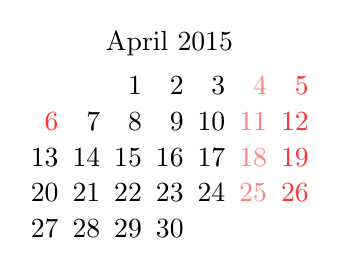
\begin{tikzpicture}[scale=1,inner sep=0.4mm]
\calendar
[dates=2015-04-01 to 2015-04-30,week list,
month label above centered,
month text={\%mt} \%y-]
if (Saturday) [red!50]
if (Sunday) [red!80]
if (equals=2015-04-06) [red!80];

\end{tikzpicture}

\end{document}